\documentclass{standalone}
\usepackage{tikz}
\usetikzlibrary{patterns, positioning}
\usepackage[sfdefault]{ClearSans} %% option 'sfdefault' activates Clear Sans as the default text font
\usepackage[T1]{fontenc}

\begin{document}
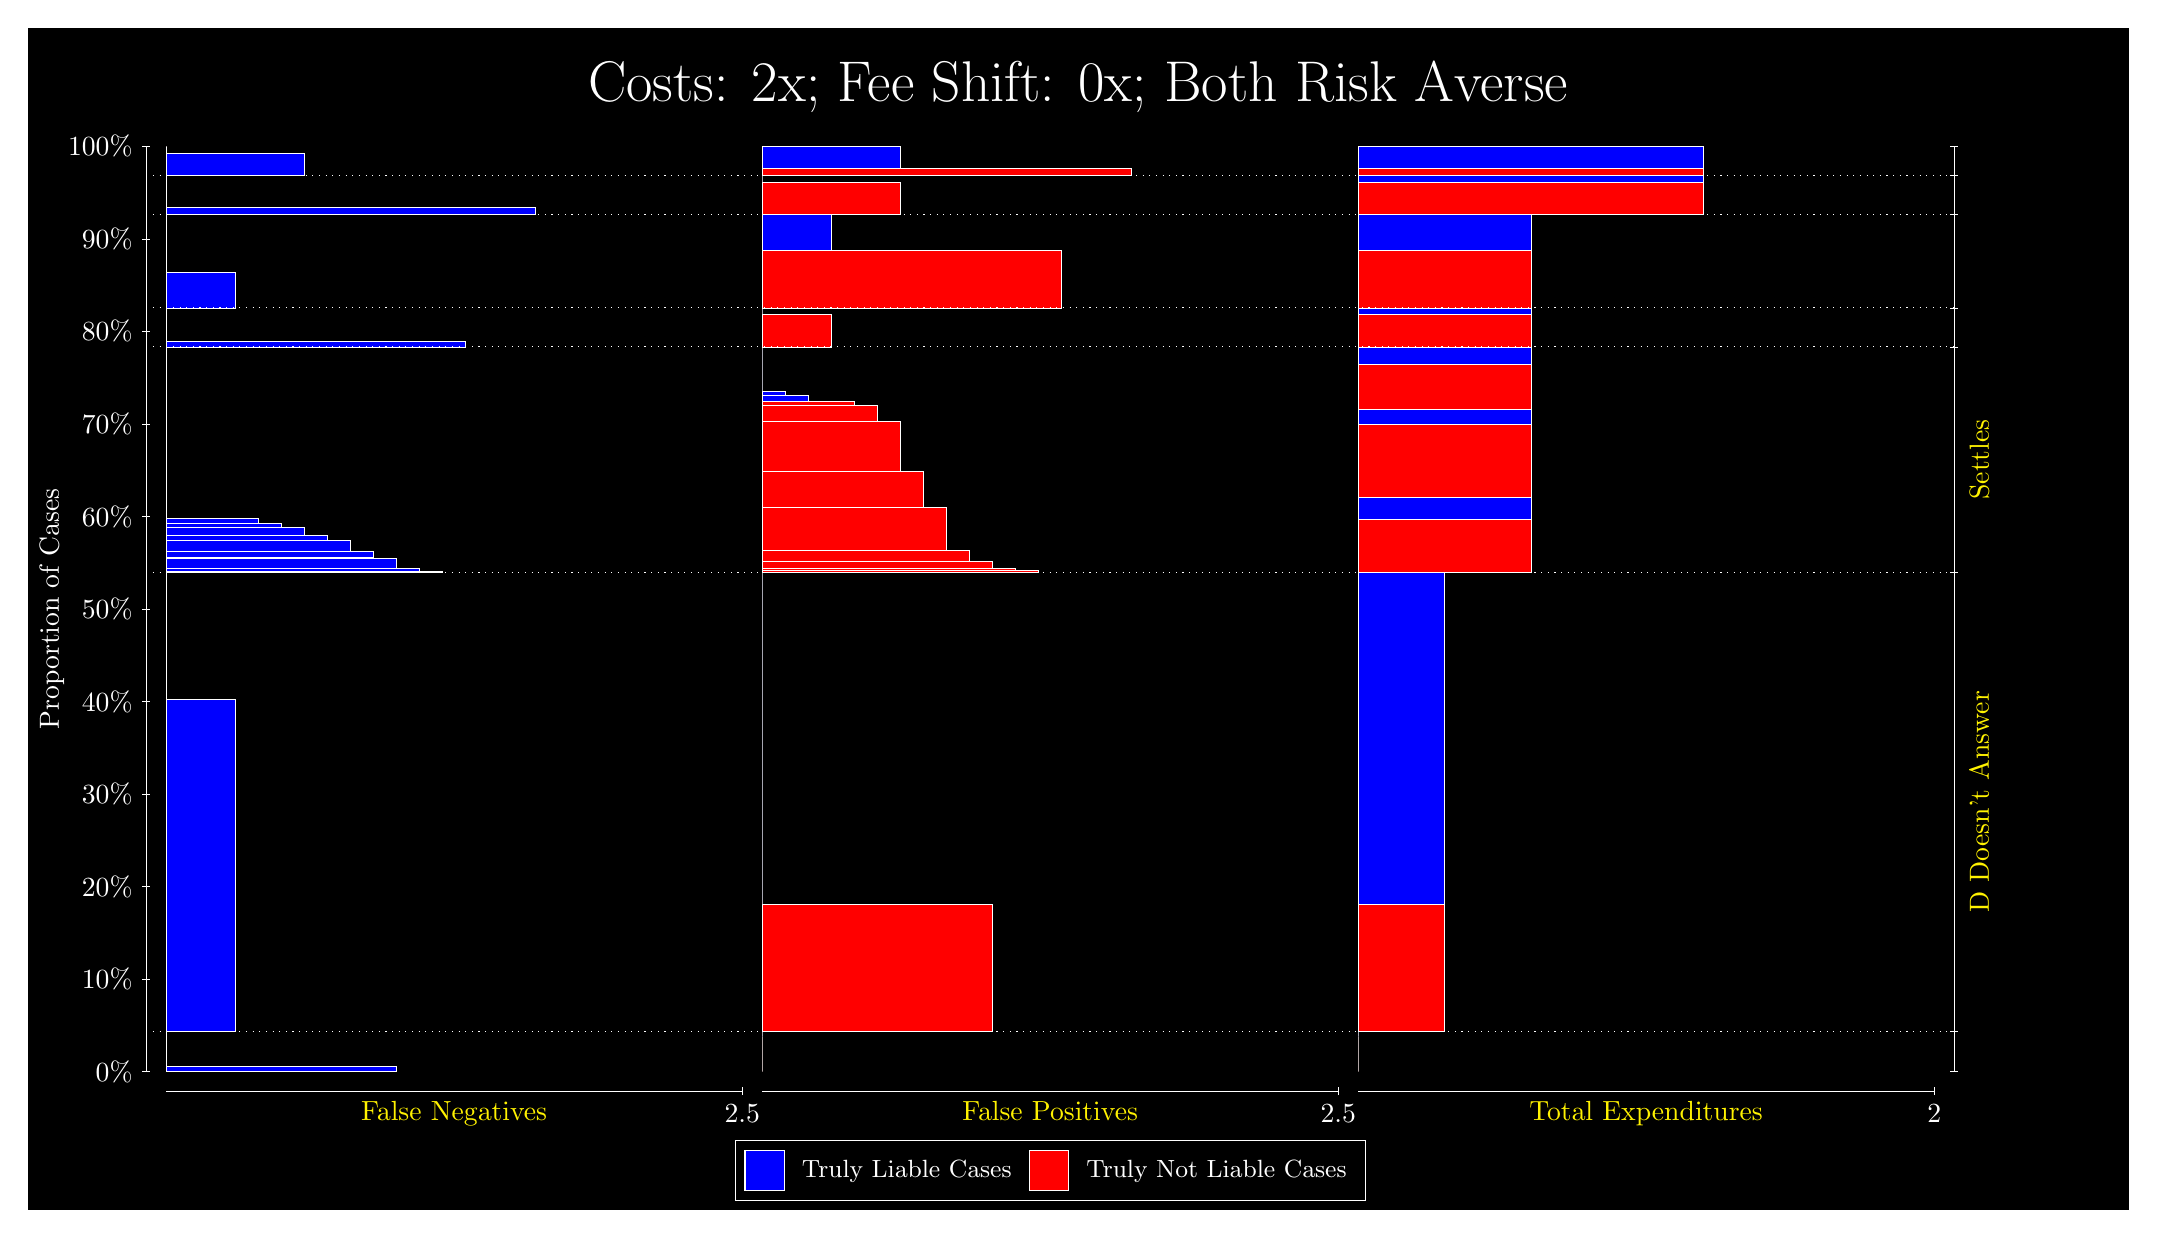
\begin{tikzpicture}
\draw[fill=black] (0,0) rectangle (26.667,15);
\draw[text=white] (0,13.5) rectangle (26.667,15) node[midway] {\huge Costs: 2x; Fee Shift: 0x; Both Risk Averse};
\draw[white, very thin] (1.5,1.75) -- (1.5,13.5);
\node[rotate=90, text=white, anchor=center] at (0.3, 7.625) {Proportion of Cases};
\draw[white, very thin] (1.45,1.75) -- (1.55,1.75);
\node[text=white, anchor=east] at (1.45, 1.75) {0\%};
\draw[white, very thin] (1.45,2.925) -- (1.55,2.925);
\node[text=white, anchor=east] at (1.45, 2.925) {10\%};
\draw[white, very thin] (1.45,4.1) -- (1.55,4.1);
\node[text=white, anchor=east] at (1.45, 4.1) {20\%};
\draw[white, very thin] (1.45,5.275) -- (1.55,5.275);
\node[text=white, anchor=east] at (1.45, 5.275) {30\%};
\draw[white, very thin] (1.45,6.45) -- (1.55,6.45);
\node[text=white, anchor=east] at (1.45, 6.45) {40\%};
\draw[white, very thin] (1.45,7.625) -- (1.55,7.625);
\node[text=white, anchor=east] at (1.45, 7.625) {50\%};
\draw[white, very thin] (1.45,8.8) -- (1.55,8.8);
\node[text=white, anchor=east] at (1.45, 8.8) {60\%};
\draw[white, very thin] (1.45,9.975) -- (1.55,9.975);
\node[text=white, anchor=east] at (1.45, 9.975) {70\%};
\draw[white, very thin] (1.45,11.15) -- (1.55,11.15);
\node[text=white, anchor=east] at (1.45, 11.15) {80\%};
\draw[white, very thin] (1.45,12.325) -- (1.55,12.325);
\node[text=white, anchor=east] at (1.45, 12.325) {90\%};
\draw[white, very thin] (1.45,13.5) -- (1.55,13.5);
\node[text=white, anchor=east] at (1.45, 13.5) {100\%};

\draw[white, very thin] (24.457,1.75) -- (24.457,13.5);
\draw[white, very thin] (24.407,1.75) -- (24.507,1.75);
\node[anchor=west] at (24.407, 1.75) {};
\draw[white, very thin] (24.407,2.2619) -- (24.507,2.2619);
\node[anchor=west] at (24.407, 2.2619) {};
\draw[white, very thin] (24.407,8.0894) -- (24.507,8.0894);
\node[anchor=west] at (24.407, 8.0894) {};
\draw[white, very thin] (24.407,10.954) -- (24.507,10.954);
\node[anchor=west] at (24.407, 10.954) {};
\draw[white, very thin] (24.407,11.448) -- (24.507,11.448);
\node[anchor=west] at (24.407, 11.448) {};
\draw[white, very thin] (24.407,12.636) -- (24.507,12.636);
\node[anchor=west] at (24.407, 12.636) {};
\draw[white, very thin] (24.407,13.135) -- (24.507,13.135);
\node[anchor=west] at (24.407, 13.135) {};
\draw[white, very thin] (24.407,13.5) -- (24.507,13.5);
\node[anchor=west] at (24.407, 13.5) {};

\draw[white, very thin, fill=blue] (1.75,1.75) rectangle (4.6775,1.8194);
\draw[white, very thin, fill=red] (1.75,1.8194) rectangle (1.75,2.2619);
\draw[white, very thin, fill=blue] (1.75,2.2619) rectangle (2.6283,6.4793);
\draw[white, very thin, fill=red] (1.75,6.4793) rectangle (1.75,8.0894);
\draw[white, very thin, fill=blue] (1.75,8.0894) rectangle (5.2631,8.1028);
\draw[white, very thin, fill=blue] (1.75,8.1028) rectangle (4.9703,8.1408);
\draw[white, very thin, fill=blue] (1.75,8.1408) rectangle (4.6775,8.2654);
\draw[white, very thin, fill=blue] (1.75,8.2654) rectangle (4.3848,8.2803);
\draw[white, very thin, fill=blue] (1.75,8.2803) rectangle (4.3848,8.3634);
\draw[white, very thin, fill=blue] (1.75,8.3634) rectangle (4.092,8.4996);
\draw[white, very thin, fill=blue] (1.75,8.4996) rectangle (3.7993,8.56);
\draw[white, very thin, fill=blue] (1.75,8.56) rectangle (3.5065,8.6594);
\draw[white, very thin, fill=blue] (1.75,8.6594) rectangle (3.2138,8.7065);
\draw[white, very thin, fill=blue] (1.75,8.7065) rectangle (2.921,8.7815);
\draw[white, very thin, fill=red] (1.75,8.7815) rectangle (1.75,10.954);
\draw[white, very thin, fill=blue] (1.75,10.954) rectangle (5.5558,11.029);
\draw[white, very thin, fill=red] (1.75,11.029) rectangle (1.75,11.448);
\draw[white, very thin, fill=blue] (1.75,11.448) rectangle (2.6283,11.903);
\draw[white, very thin, fill=red] (1.75,11.903) rectangle (1.75,12.636);
\draw[white, very thin, fill=blue] (1.75,12.636) rectangle (6.4341,12.724);
\draw[white, very thin, fill=red] (1.75,12.724) rectangle (1.75,13.135);
\draw[white, very thin, fill=blue] (1.75,13.135) rectangle (3.5065,13.413);
\draw[white, very thin, fill=red] (1.75,13.413) rectangle (1.75,13.5);
\draw[white, very thin, fill=red] (9.3189,1.75) rectangle (9.3189,2.1925);
\draw[white, very thin, fill=blue] (9.3189,2.1925) rectangle (9.3189,2.2619);
\draw[white, very thin, fill=red] (9.3189,2.2619) rectangle (12.246,3.872);
\draw[white, very thin, fill=blue] (9.3189,3.872) rectangle (9.3189,8.0894);
\draw[white, very thin, fill=red] (9.3189,8.0894) rectangle (12.832,8.1159);
\draw[white, very thin, fill=red] (9.3189,8.1159) rectangle (12.539,8.1406);
\draw[white, very thin, fill=red] (9.3189,8.1406) rectangle (12.246,8.233);
\draw[white, very thin, fill=red] (9.3189,8.233) rectangle (11.954,8.3654);
\draw[white, very thin, fill=red] (9.3189,8.3654) rectangle (11.661,8.9204);
\draw[white, very thin, fill=red] (9.3189,8.9204) rectangle (11.368,9.3702);
\draw[white, very thin, fill=red] (9.3189,9.3702) rectangle (11.075,10.004);
\draw[white, very thin, fill=red] (9.3189,10.004) rectangle (10.783,10.205);
\draw[white, very thin, fill=red] (9.3189,10.205) rectangle (10.49,10.262);
\draw[white, very thin, fill=blue] (9.3189,10.262) rectangle (9.9044,10.337);
\draw[white, very thin, fill=blue] (9.3189,10.337) rectangle (9.6116,10.384);
\draw[white, very thin, fill=blue] (9.3189,10.384) rectangle (9.3189,10.954);
\draw[white, very thin, fill=red] (9.3189,10.954) rectangle (10.197,11.373);
\draw[white, very thin, fill=blue] (9.3189,11.373) rectangle (9.3189,11.448);
\draw[white, very thin, fill=red] (9.3189,11.448) rectangle (13.125,12.181);
\draw[white, very thin, fill=blue] (9.3189,12.181) rectangle (10.197,12.636);
\draw[white, very thin, fill=red] (9.3189,12.636) rectangle (11.075,13.047);
\draw[white, very thin, fill=blue] (9.3189,13.047) rectangle (9.3189,13.135);
\draw[white, very thin, fill=red] (9.3189,13.135) rectangle (14.003,13.222);
\draw[white, very thin, fill=blue] (9.3189,13.222) rectangle (11.075,13.5);
\draw[white, very thin, fill=red] (16.888,1.75) rectangle (16.888,2.1925);
\draw[white, very thin, fill=blue] (16.888,2.1925) rectangle (16.888,2.2619);
\draw[white, very thin, fill=red] (16.888,2.2619) rectangle (17.986,3.872);
\draw[white, very thin, fill=blue] (16.888,3.872) rectangle (17.986,8.0894);
\draw[white, very thin, fill=red] (16.888,8.0894) rectangle (19.083,8.7615);
\draw[white, very thin, fill=blue] (16.888,8.7615) rectangle (19.083,9.0443);
\draw[white, very thin, fill=red] (16.888,9.0443) rectangle (19.083,9.9713);
\draw[white, very thin, fill=blue] (16.888,9.9713) rectangle (19.083,10.162);
\draw[white, very thin, fill=red] (16.888,10.162) rectangle (19.083,10.736);
\draw[white, very thin, fill=blue] (16.888,10.736) rectangle (19.083,10.954);
\draw[white, very thin, fill=red] (16.888,10.954) rectangle (19.083,11.373);
\draw[white, very thin, fill=blue] (16.888,11.373) rectangle (19.083,11.448);
\draw[white, very thin, fill=red] (16.888,11.448) rectangle (19.083,12.181);
\draw[white, very thin, fill=blue] (16.888,12.181) rectangle (19.083,12.636);
\draw[white, very thin, fill=red] (16.888,12.636) rectangle (21.279,13.047);
\draw[white, very thin, fill=blue] (16.888,13.047) rectangle (21.279,13.135);
\draw[white, very thin, fill=red] (16.888,13.135) rectangle (21.279,13.222);
\draw[white, very thin, fill=blue] (16.888,13.222) rectangle (21.279,13.5);
\draw[white, dotted] (1.5,2.2619) -- (24.457,2.2619);
\draw[white, dotted] (1.5,8.0894) -- (24.457,8.0894);
\draw[white, dotted] (1.5,10.954) -- (24.457,10.954);
\draw[white, dotted] (1.5,11.448) -- (24.457,11.448);
\draw[white, dotted] (1.5,12.636) -- (24.457,12.636);
\draw[white, dotted] (1.5,13.135) -- (24.457,13.135);
\draw[white, very thin] (1.75,1.5) -- (9.0689,1.5);
\node[text=yellow, anchor=north] at (5.4094, 1.5) {False Negatives};
\draw[white, very thin] (9.0689,1.45) -- (9.0689,1.55);
\node[text=white, anchor=north] at (9.0689, 1.45) {2.5};

\draw[white, very thin] (9.3189,1.5) -- (16.638,1.5);
\node[text=yellow, anchor=north] at (12.978, 1.5) {False Positives};
\draw[white, very thin] (16.638,1.45) -- (16.638,1.55);
\node[text=white, anchor=north] at (16.638, 1.45) {2.5};

\draw[white, very thin] (16.888,1.5) -- (24.207,1.5);
\node[text=yellow, anchor=north] at (20.547, 1.5) {Total Expenditures};
\draw[white, very thin] (24.207,1.45) -- (24.207,1.55);
\node[text=white, anchor=north] at (24.207, 1.45) {2};


\node[text=yellow, centered, rotate=90] at (24.777, 5.1756) {D Doesn't Answer};
\node[text=yellow, centered, rotate=90] at (24.777, 9.5219) {Settles};





\draw (12.978300999999998,1.5) node[draw=none] (baseCoordinate) {};
\begin{scope}[align=center]
        \matrix[scale=0.5, draw=white, below=0.5cm of baseCoordinate, nodes={draw}, column sep=0.1cm]{
            \node[rectangle, draw, minimum width=0.5cm, minimum height=0.5cm, fill=blue] {}; &
            \node[draw=none, font=\small, text=white] (B) {Truly Liable Cases}; &
            \node[rectangle, draw, minimum width=0.5cm, minimum height=0.5cm, fill=red] {}; &
            \node[draw=none, font=\small, text=white] (B) {Truly Not Liable Cases}; \\
            };
\end{scope}

\end{tikzpicture}
\end{document}